\chapter{Proceso Buscar un Usuario}
	Este capítulo explica el proceso que se lleva a cabo para buscar
	un determinado usuario en el sistema, y así mostrar los siguientes datos:
	
	\begin{itemize}
	\item Nombre
	\item Institución
	\item Rol
	\item Tipo
	\item Estado
	\item Fecha de Expiración
	
	\end{itemize}
	
	Se tiene la interfaz de bienvenida:
	\begin{figure}[hbtp]
		
		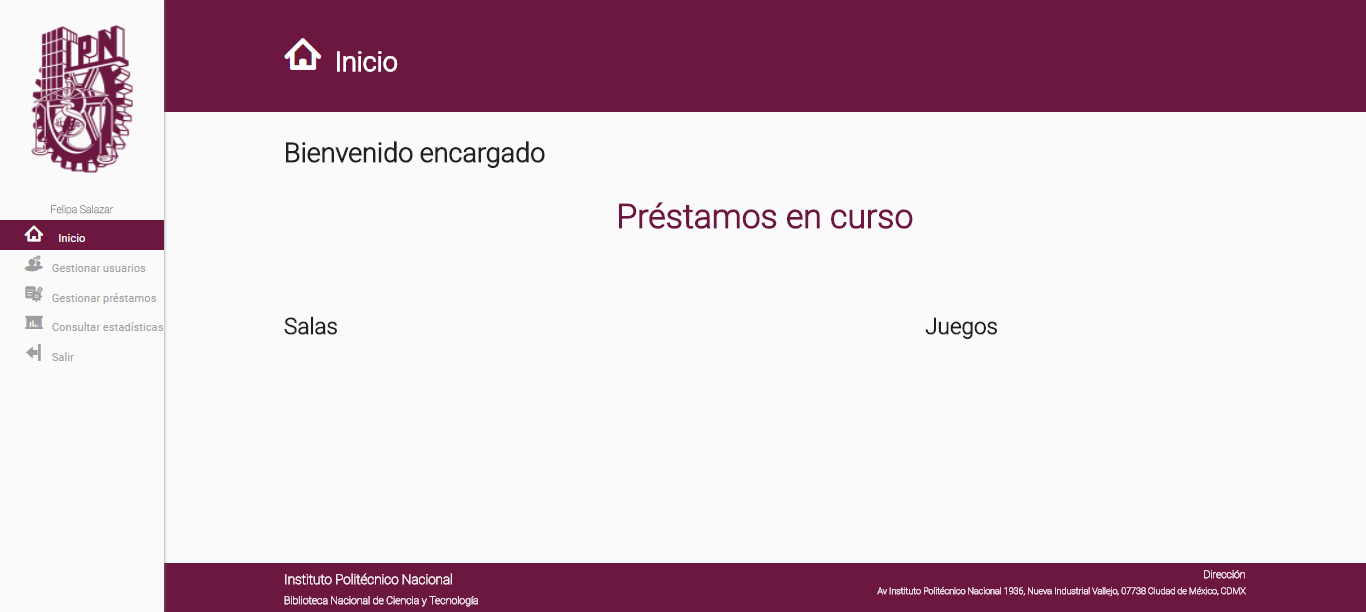
\includegraphics[scale=0.3]{images/Interfaz/IUGS02_binevenida.png}
		\caption{Bienvenida Encargado}
	\end{figure}

%%

\section{Paso 1.Bienvenida}
	\subsection{Información del usuario}

\subsection{Información de los préstamos}

\subsection{Información de la encuesta}


\section{Paso 2. Gestionar Usuario}
	Se ingresa el identificador a ser buscado.
\subsection{Subpaso 1-A: Buscar }
\begin{enumerate}
	\item Ingrese identificador.
	\item Presione el botón \textbf{Buscar}. Este paso puede derivar
		al error \textbf{Error E1-A}.

\end{enumerate}

\begin{figure}[hbtp]
		\centering
		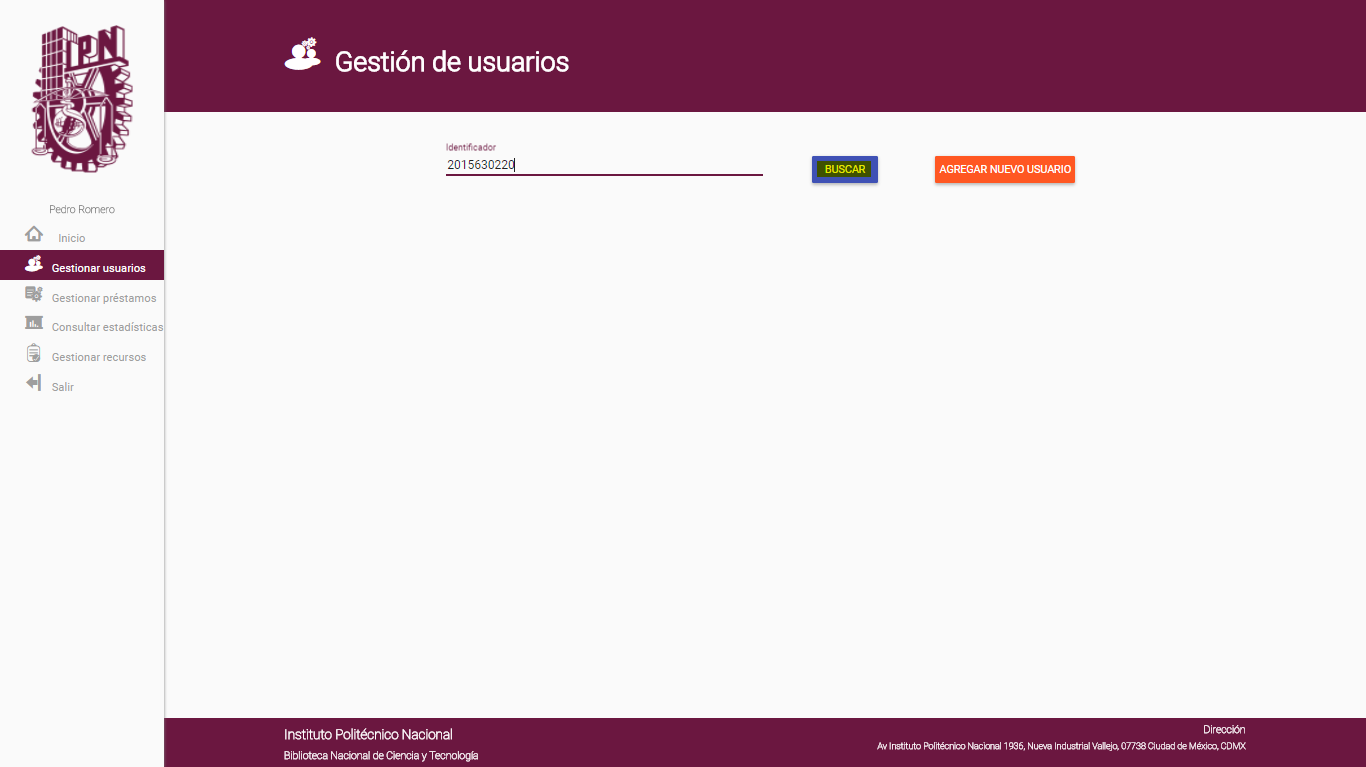
\includegraphics[scale=0.3]{images/Interfaz/IUGS22_gestionarUsuarioBuscar.png}
		\caption{Gestionar Usuario}
	\end{figure}

\subsection{Error E1-A: usuario no encontrado}
El identificador que se ingresó no se encuentra  en el sistema,
debe verificarlo.
\begin{itemize}
	\item Presionar \textbf{Aceptar} en la ventana emergente 
		\textbf{MAT-48 Usuario no encontrado}
		%\begin{figure}[hbtp]
		
		%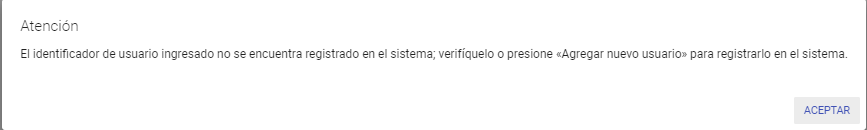
\includegraphics[scale=0.3]{images/Interfaz/MAT48_usuarioNoEncontrado.png}
		%\caption{Gestionar Usuario}

    %%
    %% ¡Esta imágen no existe!
    %% Favor de no subir algo que interrumpa la compilación.
    %% RQF7
    %%
    %% La terminación del archivo es (.PNG)
    %%
	%\end{figure} 
\end{itemize}

	
\section{Paso 3. Resultado}
	Resultado de la búsqueda según el identificador proporcionado con los datos

\subsection{Subpaso 2-A: Solicitante}
\begin{enumerate}
	\item Nombre
	\item Institución
	\item Rol
	\item Tipo
	\item Estado
	\item Fecha de Expiración
	
		\begin{figure}[hbtp]
		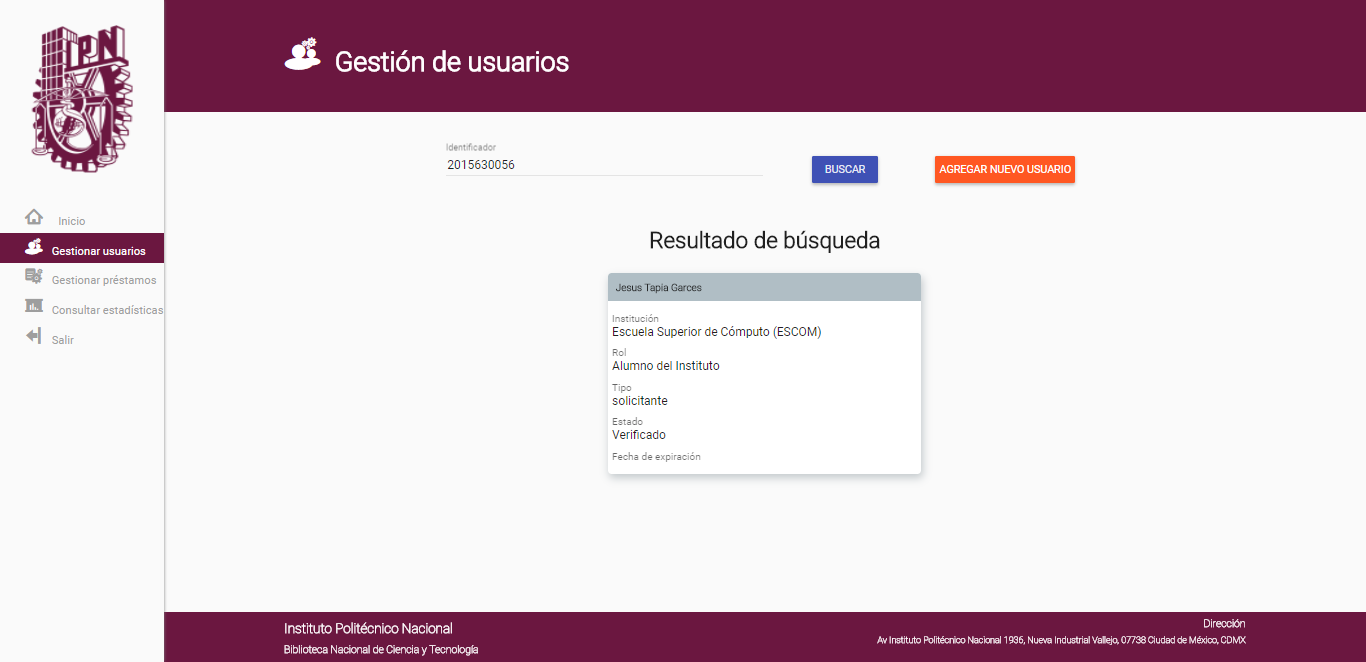
\includegraphics[scale=0.3]
		{images/Interfaz/IUGS22_EncargadoBusquedaSolicitante.png}
		\caption{Busqueda de un Solicitante}
	\end{figure}
\end{enumerate}

\subsection{Subpaso 2-B: Encargado o Administrador}
\begin{enumerate}
	\item Nombre
	\item Institución
	\item Rol
	\item Tipo
	\item Estado
	\item Fecha de Expiración
	
	\begin{figure}[hbtp]
		
		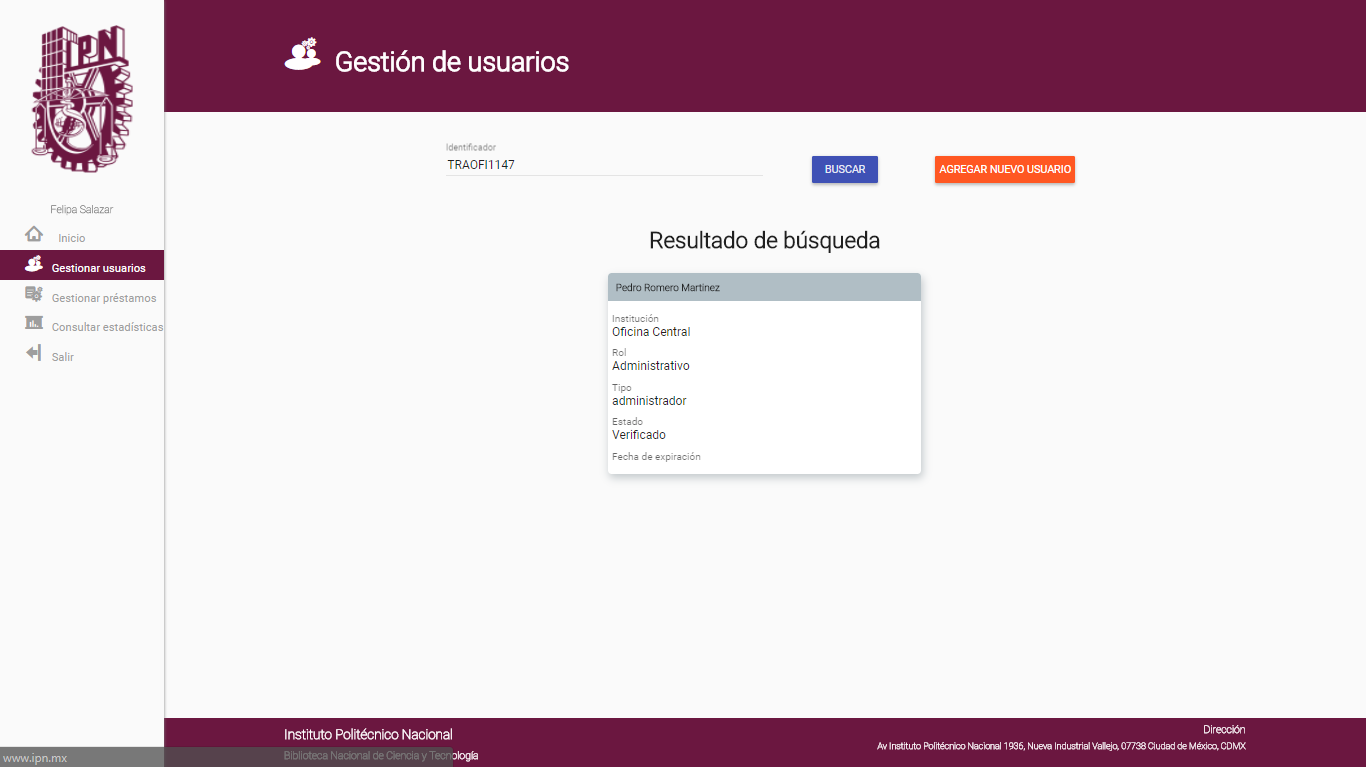
\includegraphics[scale=0.3]
		{images/Interfaz/IUGS22_EncargadoBusquedaEncargado.png}
		\caption{Busqueda de un Encargado}
	\end{figure} 
\end{enumerate}

	